\section{情報2(木村)}
\noindent\begin{tabular}{|c|} % 問題1
  \hline
  問題1 \\
  \hline
\end{tabular}
次の各問いに答えよ．各2点(計64点)\\
(01) 2進数で示された「1011~0111」を10進数に変換して答えよ．\\
(02)2進数の加算「1101~0110 + 1011~1001」の計算結果を10進数に変換して答えよ．\\
(03)16進数で示された「246」を10進数に変換して答えよ．\\
(04)10進数で示した次の数値のうち「2進数による有限小数」で表現できるものをすべて答えよ．\par\quad
\ding{172}0.4\quad \ding{173}0.75\quad \ding{174}0.1\quad \ding{175}0.3125\quad \ding{176}0.5\quad \ding{177}0.25\\
(05)10進数の「-6」を2進数に変換して答えよ．なお，負数は補数表現を使ってあらわすものとして，また値を格納\par\quad するメモリは4ビットを想定すること．\\
(06)8ビットの2進数「1010~0000」の補数を答えよ．\\
(07)非負の整数値を8ビットのメモリで扱うコンピュータを考える．このコンピュータを使って10進数の計算「182\par\quad+ 74」を実行したとき，得られる結果を10進数で答えよ(オーバーフローが生じることを考慮して答えること)．\\
(08)ある実験装置の出力値を10回計測した．出力値の平均を求めたところ8.9であった．このとき，3回目に計測\par\quad された出力値10.7の「偏差」はいくらか答えよ．\\
(09)Excelにおける指数表示「3.638E + 04」を，通常の数値表示にしたときの値を答えよ．\\
(10)指定した範囲の一様乱数(整数)の生成に使われるExcel関数を答えよ．\\
(11)USBメモリは「主記憶装置」と「補助記憶装置」のどちらに分類されるか答えよ．\\
(12)相対的に製造コストが低く，大きな記憶容量を持ったRAMが求められるとき，それに適するものはSRAMと\par\quad DRAMのどちらか答えよ．\\
(13)「HDD(Hard Disk Drive)は半導体メモリである」は，適切な説明と「言える」か「言えない」か答えよ．\\
(14)コンピュータ内部において，CPUとメモリの間やCPUと入出力装置の間などで，データを受け渡す役割をす\par\quad るものを答えよ．\\
(15)次に示すRGB値のうち「黒色」を表すものはどれか答えよ．最も適切なものを記号で答えよ．\par\quad
\ding{172}(0, 255, 255)\quad \ding{173}(255, 0, 255)\quad \ding{174}(255, 255, 0)\quad \ding{175}(255, 255, 255)\quad \ding{176}(0, 0, 0)\\
(16)無圧縮形式で画素数(縦横のピクセル数)が同じ場合，フルカラー画像は，256階調グレースケール画像の約何倍\par\quad のファイルサイズになるか答えよ．\\
(17)以下の代表的な画像形式について，不可逆圧縮である画像形式をすべて答えよ．\par\quad
\ding{172}jpg(jpeg)\quad \ding{173}png\quad \ding{174}heic/heif\quad \ding{175}bmp\quad \ding{176}gif\\
(18)PhotoshopやIllustrator，Premiere Proなどのソフトウェアを開発・販売している企業は，次のうちどれか，記\par\quad 号で答えよ．\par\quad
\ding{172}Microsoft\quad \ding{173}Apple\quad \ding{174}NVIDIA\quad \ding{175}Adobe\quad \ding{176}Macromedia\quad \ding{177}Corel\\
(19)256階調のグレースケール画像において，1画素あたりの輝度を表現するために必要なデータ量は何bitか答え\par\quad よ．\\
(20)CIDR表記で「192.168.100.129/8」のとき，このサブネットマスクを10進数による表記で答えよ．\\
(21)Windowsのエクスプローラにおいて，連続しない複数のファイルを選択したい．範囲先頭のファイルをクリック\par\quad 選択した後，範囲末尾のファイルをクリック選択する際に押下すべきキーはどれか，記号で答えよ．\par\quad
\ding{172}alt\quad \ding{173}Shift\quad \ding{174}Ctrl\quad \ding{175}Tab\quad \ding{176}esc\\
(22)Windowsにおいて，IPアドレスなどのネットワーク設定の詳細情報を表示(確認)するためのコマンドを答え\par\quad よ．なお，この問題の解答では，半角スペースを\textvisiblespace の記号を使って示すこと．\\
(23)Windowsにおいて「エクスプローラ」を起動するためのショートカットキーはどれか答えよ．記号で答えよ．\par\quad
\ding{172}Win + E\quad \ding{173}Win + I\quad \ding{174}Win + W\quad \ding{175}Win + R\quad \ding{176}Win + F\\
(24)一般的な構成のノートPC(Windows 11)にUSBメモリを接続した．このUSBメモリは何ドライブとしてOS\par\quad に認識される可能性が高いか，記号で答えよ．なお，USBメモリ以外，PCにリムーバブルメディアは接続され\par\quad ていないものとする．\par\quad
\ding{172}Aドライブ\quad \ding{173}Bドライブ\quad \ding{174}Cドライブ\quad \ding{175}Dドライブ\quad \ding{176}OneDrive\\
(25)ICT分野における「LAN」とは何の頭文字をとったものか英語で答えよ．\\
(26)DNSの機能について説明しているものはどれか．最も適切なものを記号で答えよ．\par\quad
\ding{172}ネットワーク接続に際してユーザー認証をする．\par\quad
\ding{173}ネットワークに接続されたデバイスを識別する．\par\quad
\ding{174}ドメイン名とIPアドレスを対応付ける．\par\quad
\ding{175}セグメント間の通信パケットを監視・管理する．\\
(27)TCP/IP において通信相手が「同一セグメントに存在するかどうか」は，どのような情報によって判断できるか．\par\quad 最も適切なものを記号で答えよ．\par\quad
\ding{172}相手の「IPアドレス」，デフォルトゲートウェイの「IPアドレス」\par\quad
\ding{173}相手の「IPアドレス」，自分の「IPアドレス」，自分の「サブネットマスク」\par\quad
\ding{174}相手の「IPアドレス」，自分の「IPアドレス」，デフォルトゲートウェイの「IPアドレス」\par\quad
\ding{175}相手の「IPアドレス」，相手の「サブネットマスク」，自分の「IPアドレス」\\
(28)ネットワークに接続するデバイスにおいて，デフォルトゲートウェイが正しく設定されていない場合，どのような状況となるか．最も適切なものを記号で答えよ．\par\quad
\ding{172}インターネットへの接続が不可能になる．\par\quad
\ding{173}同一セグメント内のデバイスと通信ができなくなる．\par\quad
\ding{174}他セグメントにあるデバイスと通信ができなくなる．\par\quad
\ding{175}全てのデバイスと通信ができなくなる．\\
(29)インターネット全体で重複しないように一意に割り当てる必要があるのは「グローバルIPアドレス」と「プライ\par\quad ベートIPアドレス」のどちらか答えよ．\\
(30)次の運用のうち，ネットワーク経由のハッキングを受ける危険性が最も低いものはどれか．\par\quad
\ding{172}スタンドアロン\quad \ding{173}閉じた LAN に接続\quad \ding{174}インターネットに接続した LAN に接続\\
(31)Excelにおいて，範囲A1:E1の平均値を計算し，小数点第1位を切り上げた値(すなわち整数値)をセルF1に得\par\quad たい．セルF1に記述すべきExcel関数を答えよ．\\
(32)次の文章の括弧にあてはまる最も適切な言葉を漢字3文字で答えよ．「統計学では(\quad\quad\quad)から抽出した部分集\par\quad 合を標本という」\\

\noindent\begin{tabular}{|c|} % 問題2
  \hline
  問題2 \\
  \hline
\end{tabular}
次の\textbf{設定}を読み，以下の各問いに答えよ．各2点(計6点)\\
\begin{minipage}{.7\textwidth}
  \textbf{設定}\quad Windows11のPCにおいて右図のようなフォルダ構成を想定する．
  \begin{itemize}
    \item フォルダ「\textbf{1年}」の絶対パスは「\textbf{C:¥Users¥kato¥授業¥1年}」である．
    \item フォルダ「\textbf{情報2}」には，ファイル「\textbf{講義ノート01.pdf}」が存在する
    \item フォルダ「\textbf{課題}」には，ファイル「\textbf{課題\ding{172}.xlsx}」が存在する．
  \end{itemize}
(33) カレントフォルダが「\textbf{国語1}」のとき，ファイル「\textbf{課題\ding{172}.xlsx}」の絶対パス\par\qquad を答えよ．\\
(34) カレントフォルダが「\textbf{1年}」のとき，ファイル「\textbf{課題\ding{172}.xlsx}」の相対パスを\par\qquad 答えよ．なお，カレントフォルダを表す文字も省略せずに含めること．\\
\end{minipage}
\begin{minipage}{.3\textwidth}
  \hspace{0.8cm}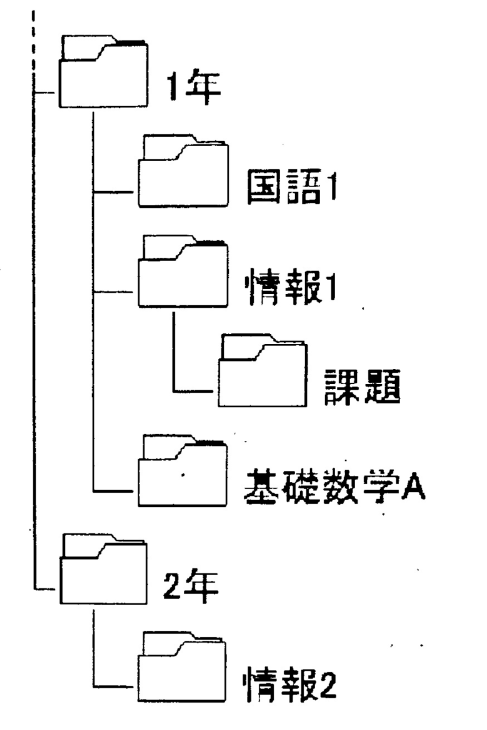
\includegraphics[width=0.7\linewidth]{image/Inf1.png}
\end{minipage}
(35) カレントフォルダが「\textbf{基礎数学A}」のとき，ファイル「\textbf{講義ノート01.pdf}」の相対パスを答えよ．なお，カレントフォルダを表す文字も省略せずに含めること．\\
\newpage

\noindent\begin{tabular}{|c|} % 問題3
  \hline
  問題3 \\
  \hline
\end{tabular}
次の各問いについて，\textbf{ア$\sim$エ}の記号で答えよ．各2点(計30点)\\
(36)文書作成ソフトや表計算ソフトなどにおいて，一連の操作手順をあらかじめ定義しておき，実行する機能はどれ\par\quad か．\par\quad
ア：オートコンプリート\quad イ：プラグアンドプレイ\quad ウ：マクロ\quad エ：ソースコード\\
(37)負の整数を「2の補数」で表現するとき，8桁の2進数で表現できる数値範囲を10進数で表したものはどれか．\par\quad
ア：-128$\sim$128\quad イ：-128$\sim$127\quad ウ：-127$\sim$128\quad エ：-127$\sim$127\\
(38)パスワードの解読方法の一つとして，全ての文字の組合せを試みる総当たり攻撃がある．"A"から"Z"の26種類\par\quad の文字を使用できるパスワードにおいて，文字数を4文字から6文字に増やすと，総当たり攻撃でパスワードを\par\quad 解読するための最大の試行回数は何倍になるか．\par\quad
ア：2\quad イ：24\quad ウ：52\quad エ：676\\
(39)Windowsにおいて，パス文字列のなかでフォルダ階層を区切るために使用する文字(記号)はどれか答えよ．\par\quad
ア：¥\quad イ：\$\quad ウ：$>$\quad エ：/\\
(40)サーバに2台のHDDを接続しているとき，HDDの故障が「どちらか片方だけ」であれば運用がつづけられる\par\quad ようにしたい．使用する構成として適切なものはどれか．\par\quad
ア：ストライピング\quad イ：ルーティング\quad ウ：テザリング\quad エ：ミラーリング\\
(41)4台のHDDを使い，障害に備えるために「1台分の容量をパリティ情報の記録に使用するRAID5」を構成する．\par\quad 1台のHDDの容量が1TBのとき，実効データ容量はおよそ何Bか．\par\quad
ア：1TB\quad イ：2TB\quad ウ：3TB\quad エ：4TB\\
(42)コンピュータハードウェアに関する文脈においてCPUとは何の略語か．次の選択肢から最も適切なものを記号\par\quad で答えよ．\par\quad
ア：Central Process Unit\par\quad
イ：Computer Processing Unit\par\quad
ウ：Central Processing Unit\par\quad
エ：Control Processing Unit\\
(43)スマートフォンなどのタッチパネルで広く採用されている方式であり，指がタッチパネルの表面に近づいたとき\par\quad に，その位置を検出する方式はどれか．\par\quad
ア：感圧式\quad イ：静電容量方式\quad ウ：電磁誘導方式\quad エ：光学式\\
(44)スキャナを使ってカラー写真のデジタル化を行う．このスキャナは解像度が300dpiで24ビットカラーの画像を\par\quad 取り込むことができる．データ圧縮を全く行わないとき，15cm$\times$10cmのカラー写真を1枚保存するためのディ\par\quad スク容量は，およそ何Mバイトか．ここでは，1(inch) = 2.5(cm)とし，1M=10の6乗とする．\par\quad 
ア：約 2MB\quad イ：約 3.5MB\quad ウ：約 5MB\quad エ：約 6.5MB\\
(45)IoTデバイスとIoTサーバで構成され，IoTデバイスが計測した外気温をIoTサーバへ送り，IoTサーバからの\par\quad 指示で窓を開閉するシステムがある．このシステムのIoTデバイスに搭載されて，窓を開閉する役割を持つもの\par\quad はどれか．\par\quad
ア：アクチュエータ\par\quad
イ：エッジコンピューティング\par\quad
ウ：キャリアアグリゲーション\par\quad
エ：センサ\\
(46)ネットワークに関する次の記述中のa$\sim$cに入れる字句の適切な組合せはどれか．\par\quad
建物内などの狭い範囲で構成されるネットワークは
\noindent\begin{tabular}{|c|}
  \hline
  a \\
  \hline
\end{tabular}
と呼ばれ，地域的に離れた地点を結ぶネットワークは\par\quad
\noindent\begin{tabular}{|c|}
  \hline
  b \\
  \hline
\end{tabular}
と呼ばれる．インターネット上で一意に割り当てられるIPアドレスは
\noindent\begin{tabular}{|c|}
  \hline
  c \\
  \hline
\end{tabular}
である．\par\quad
ア：
\noindent\begin{tabular}{|c|}
  \hline
  a \\
  \hline
\end{tabular}
LAN，
\noindent\begin{tabular}{|c|}
  \hline
  b \\
  \hline
\end{tabular}
WAN，
\noindent\begin{tabular}{|c|}
  \hline
  c \\
  \hline
\end{tabular}
グローバルIPアドレス\par\quad
イ：
\noindent\begin{tabular}{|c|}
  \hline
  a \\
  \hline
\end{tabular}
WAN，
\noindent\begin{tabular}{|c|}
  \hline
  b \\
  \hline
\end{tabular}
LAN，
\noindent\begin{tabular}{|c|}
  \hline
  c \\
  \hline
\end{tabular}
プライベートIPアドレス\par\quad
ウ：
\noindent\begin{tabular}{|c|}
  \hline
  a \\
  \hline
\end{tabular}
LAN，
\noindent\begin{tabular}{|c|}
  \hline
  b \\
  \hline
\end{tabular}
WAN，
\noindent\begin{tabular}{|c|}
  \hline
  c \\
  \hline
\end{tabular}
プライベートIPアドレス\par\quad
エ：
\noindent\begin{tabular}{|c|}
  \hline
  a \\
  \hline
\end{tabular}
WAN，
\noindent\begin{tabular}{|c|}
  \hline
  b \\
  \hline
\end{tabular}
LAN，
\noindent\begin{tabular}{|c|}
  \hline
  c \\
  \hline
\end{tabular}
グローバルIPアドレス\\\newpage
(47)サブネットマスクの役割として，適切なものはどれか．\par\quad
ア：IPアドレスからEthernet上のMACアドレスを割り出す．\par\quad
イ：通信相手先の「ドメイン名」と「IPアドレス」を対応付ける．\par\quad
ウ：インターネットと内部ネットワークを中継するときの「グローバルIPアドレス」と「プライベートIPアド\par\quad\quad\quad レス」を対応付ける．\par\quad
エ：IPアドレスに含まれる「ネットワークアドレス」と，そのネットワークに属する個々のコンピュータの「ホ\par\quad\quad\quad ストアドレス」を区分する．\\
(48)表計算ソフトを用いて2つの科目XとYの点数を評価して合否判定をする．それぞれの点数はワークシートの\par\quad セルA2とB2に入力する．合格判定条件\ding{172}または\ding{173}に該当するときはセルC2に「合格」，それ以外のときは\par\quad「不合格」を表示したい．セルC2に入力すべき式はどれか．\par\:
〔合格判定条件〕\par\quad\:
\ding{172} 科目Xと科目Yの合計が150点以上である．\par\quad\:
\ding{173} 科目Xと科目Yがともに70点以上である．\vspace{0.2cm}\\\hspace{0.8cm}
  \renewcommand{\arraystretch}{0.8}
  \noindent\begin{tabular}{|A|
    >{\centering\arraybackslash}m{0.09\linewidth}|
    *{3}{>{\centering\arraybackslash}m{0.09\linewidth}|}
  }
  \rowcolor[gray]{0.8}
    \hline
    & A & B & C \\ \hline
    1 & 科目X & 科目Y & 合否 \\ \hline
    2 & 50 & 80 &  \\ \hline
  \end{tabular}
\vspace{0.2cm}
\par\:
ア：IF(論理和((A2+B2)≧150, 最大(A2, B2)≧70), '合格', '不合格')\par\:
イ：IF(論理和((A2+B2)≧150, 最小(A2, B2)≧70), '合格', '不合格')\par\:
ウ：IF(論理積((A2+B2)≧150, 最大(A2, B2)≧70), '合格', '不合格')\par\:
エ：IF(論理積((A2+B2)≧150, 最小(A2, B2)≧70), '合格', '不合格')\\
(49)表計算ソフトを用いてワークシートに示す各商品の月別売上額データを用いた計算を行う．セルE2に式「条件付個数(\$B\$2:\$D\$2,>10000)」を入力した後，セルE3とE4に複写したとき，セルE4に表示される値はどれか．
\vspace{0.2cm}\\\hspace{2.5cm}
    \renewcommand{\arraystretch}{0.8}
    \noindent\begin{tabular}{|A|
      >{\centering\arraybackslash}m{0.09\linewidth}|
      *{5}{>{\centering\arraybackslash}m{0.12\linewidth}|}
    }
    \rowcolor[gray]{0.8}
      \hline
      & A & B & C & D & E \\ \hline
      1 & 商品名 & 1月売上額 & 2月売上額 & 3月売上額 & 条件付個数 \\ \hline
      2 & 商品A & 30,000 & 15,000 & 20,000 & \\ \hline
      3 & 商品B & 5,000 & 10,000 & 5,000 & \\ \hline
      4 & 商品C & 10,000 & 20,000 & 10,000 & \\ \hline
    \end{tabular}
  \vspace{0.2cm}
\par\:
ア：0\quad イ：1\quad ウ：2\quad エ：3\\
(50)水田の水位を計算することによって，水田の水門を自動的に開閉するIoTシステムがある．図中の
\noindent\begin{tabular}{|c|}
  \hline
  a \\
  \hline
\end{tabular}
，
\noindent\begin{tabular}{|c|}
  \hline
  b \\
  \hline
\end{tabular}
に入れる字句の適切な組合せはどれか．\\
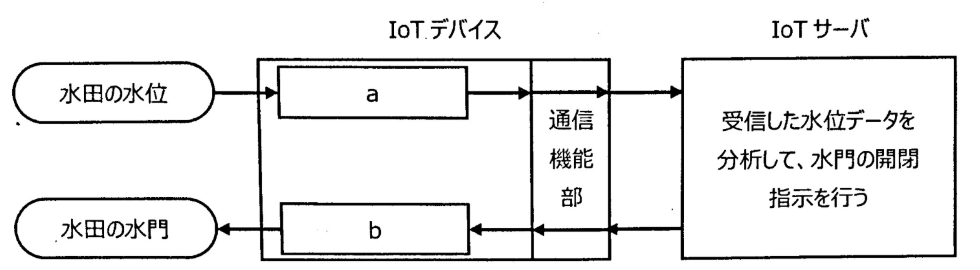
\includegraphics[width=\linewidth]{image/Inf2.png}

\par\quad ア：
\noindent\begin{tabular}{|c|}
  \hline
  a \\
  \hline
\end{tabular}
アクチュエータ
\noindent\begin{tabular}{|c|}
  \hline
  b \\
  \hline
\end{tabular}
IoTゲートウェイ\par\quad
イ：
\noindent\begin{tabular}{|c|}
  \hline
  a \\
  \hline
\end{tabular}
アクチュエータ
\noindent\begin{tabular}{|c|}
  \hline
  b \\
  \hline
\end{tabular}
センサ\par\quad
ウ：
\noindent\begin{tabular}{|c|}
  \hline
  a \\
  \hline
\end{tabular}
センサ
\noindent\begin{tabular}{|c|}
  \hline
  b \\
  \hline
\end{tabular}
IoT ゲートウェイ\par\quad
エ：
\noindent\begin{tabular}{|c|}
  \hline
  a \\
  \hline
\end{tabular}
センサ
\noindent\begin{tabular}{|c|}
  \hline
  b \\
  \hline
\end{tabular}
アクチュエータ\\



\noindent\renewcommand{\arraystretch}{1.8}
  \begin{tabular}{|m{0.33\linewidth}|m{0.33\linewidth}|m{0.33\linewidth}|}
      \hline
      \quad\quad(01)&\:\:\:(02)&\:\:\:(03) \\ \hline
      \quad\quad(04)&\:\:\:(05)&\:\:\:(06) \\ \hline
      \quad\quad(07)&\:\:\:(08)&\:\:\:(09) \\ \hline
      \quad\quad(10)&\:\:\:(11)&\:\:\:(12) \\ \hline
      \quad\quad(13)&\:\:\:(14)&\:\:\:(15) \\ \hline
      \quad\quad(16)&\:\:\:(17)&\:\:\:(18) \\ \hline
      \quad\quad(19)&\:\:\:(20)&\:\:\:(21) \\ \hline
      \quad\quad(22)&\:\:\:(23)&\:\:\:(24) \\ \hline
      \quad\quad(25)&\:\:\:(26)&\:\:\:(27) \\ \hline
      \quad\quad(28)&\:\:\:(29)&\:\:\:(30) \\ \hline
      \quad\quad(31)&\:\:\:(32)& \\ \hline
      \multicolumn{3}{|m{\linewidth}|}{(33)} \\ \hline
      \multicolumn{3}{|m{\linewidth}|}{(34)} \\ \hline
      \multicolumn{3}{|m{\linewidth}|}{(35)} \\ \hline
      \quad\quad(36)&\:\:\:(37)&\:\:\:(38) \\ \hline
      \quad\quad(39)&\:\:\:(40)&\:\:\:(41) \\ \hline
      \quad\quad(42)&\:\:\:(43)&\:\:\:(44) \\ \hline
      \quad\quad(45)&\:\:\:(46)&\:\:\:(47) \\ \hline
      \quad\quad(48)&\:\:\:(49)&\:\:\:(50) \\ \hline
    \end{tabular}